% Template for ICASSP-2026 paper; to be used with:
%          spconf.sty  - ICASSP/ICIP LaTeX style file, and
%          IEEEbib.bst - IEEE bibliography style file.
% --------------------------------------------------------------------------
\documentclass{article}
\usepackage{spconf,amsmath,graphicx,hyperref, amssymb}
\usepackage{siunitx}
% Example definitions.
% --------------------
\def\x{{\mathbf x}}
\def\L{{\cal L}}

% Title.
% ------
\title{Near-Field Holotomography Reconstruction Using Implicit Neural Representations}
%
% Single address.
% ---------------
%\name{Author(s) Name(s)\thanks{Thanks to XYZ agency for funding.}}
%\address{Author Affiliation(s)}
%
% For example:
% ------------
%\address{School\\
%	Department\\
%	Address}
%
% Two addresses (uncomment and modify for two-address case).
% ----------------------------------------------------------
\name{
	Johannes Gruen$^{1}$\thanks{We acknowledge DESY (Hamburg, Germany), a member of the Helmholtz Association HGF, for the provision of experimental facilities, and DASHH, Data Science in Hamburg - Helmholtz Graduate School  for the Structure of Matter, for financial support. Parts of this research were carried out at the PETRA III beamline P05: Beamtime-ID (11019330).
	This research was supported in part through the Maxwell computational resources operated at DESY. This research was supported by Hi-Acts, an innovation platform under the grant of the Helmholtz Association HGF.}, 
	Sebastian Eberle$^{1}$, 
	Imke Greving$^{2}$,
	Silja Flenner$^{2}$, 
	Martin Burger$^{3,4}$, 
	Christian G. Schroer$^{1,3,5}$,
	Johannes Hagemann$^{1}$
}

\address{
	$^{1}$Center for X-Ray and Nano Science CXNS, Deutsches Elektronen Synchroton DESY, \\
	$^{2}$ Institute of Materials Physics, Helmholtz-Zentrum Hereon\\
	$^{3}$Helmholtz Imaging, Deutsches Elektronen Synchroton DESY\\ 
	$^{4}$Department Mathematik, Universität Hamburg\\ 
	$^{5}$Department Physik, Universität Hamburg
}
\begin{document}
%\ninept
%
\maketitle
%
\begin{abstract}
X-ray near-field holo-tomography enables non-destructive, in-situ reconstruction of the complex refractive index at nanometer-scale resolution.
Traditionally, this process involves two separate steps: first retrieving the projected phase for different rotation angles, then applying tomographic reconstruction to obtain a 3D volume from 2D projections.
Both steps are ill-posed inverse problems and separating them leads to information loss, due to reconstruction errors.
Recent advances in implicit neural representations (INRs) have demonstrated remarkable capabilities in scene rendering and tomographic reconstruction.
In this work, we propose a unified INR-based framework that jointly solves the phase retrieval and tomographic reconstruction problems.
This joint formulation enforces 3D consistency, resulting in significantly improved phase and volumetric reconstructions.
Moreover, INRs provide substantial data compression, facilitating efficient storage and processing.
\end{abstract}
%
\begin{keywords}
X-ray near-field holo-tomography, Implicit neural representations
\end{keywords}
%
\section{Introduction}
\label{sec:intro}
X-ray computed tomography (CT) is a widely employed technique for reconstructing three-dimensional (3D) volumes from two-dimensional (2D) projection data.
Conventional CT relies on absorption contrast, which diminishes with increasing energy. 
At higher energy, however, phase contrast becomes dominant, motivating the development of X-ray near-field holography, which can be modeled using the Fresnel propagation.
This approach is particularly advantageous for weakly absorbing biological specimens, where absorption contrast is insufficient to reveal structural details, but is also used for characterization of function materials \cite{vesely3DXrayNanotomography2021a,flennerHardXrayNanoholotomography2020b,gerhardtThreedimensionalArchitectureLinearized2025,reimersDevelopmentBioreactorCoupledFlowCell2023}.

In this setting, the conventional tomographic reconstruction problem is augmented by an additional phase retrieval problem, which must be solved for each projection image.
Phase retrieval is inherently nonlinear and ill-posed, as it seeks to reconstruct the complex-valued refractive index from real-valued intensity measurements.
Furthermore, the contrast transfer function (CTF) exhibits multiple zeros, corresponding to spatial frequencies with no measurable phase information, which further exacerbates the ill-posedness of the inverse problem.

A common strategy to mitigate this limitation is to record projections at multiple propagation distances, thereby improving the phase signal, as demonstrated by Cloetens \textit{et~al.}~\cite{cloetensHolotomographyQuantitativePhase1999a}.
More recently, several studies have shown that it is possible to reconstruct the complex refractive index from measurements acquired at a single propagation distance.
This is achieved by incorporating prior knowledge, such as background constraints or the assumption of phase-only objects, which can yield accurate and stable reconstructions~\cite{doraArtifactsuppressingReconstructionStrongly2024,fienupReconstructionSupportObject1982,wittwerPhaseRetrievalFramework2022}.

An alternative approach to introducing priors is to enforce three-dimensional consistency by jointly solving the tomographic reconstruction and phase retrieval problems.
This coupling imposes a strong constraint on the recovered phase maps, effectively constraining them to be consistent with the underlying 3D structure.
For non-rotational symmetric objects joint reconstruction also reduces the loss of information due to zeros in the CTF, as the frequency changes depending on the angle, allowing the 3D reconstruction for a subset of angles, similar to sparse angle tomography.

The concept of joint 3D reconstruction is not new.
As early as 2014, Ruhland \textit{et~al.} proposed and demonstrated such an approach under the assumption of optically weak objects, for which the exponential attenuation model can be linearized~\cite{ruhlandtThreedimensionalPhaseRetrieval2014,ruhlandtThreedimensionalPropagationNearfield2016a}.
The principal limitation of this method, however, lies in its computational and memory requirements, as the reconstruction volume scales cubically with resolution.
Given that a typical detector features $2048 \times 2048$ pixels, this quickly becomes prohibitive.

A promising alternative is to represent the volume in a continuous, implicit form rather than on a discrete voxel grid~\cite{mildenhallNeRFRepresentingScenes2020a}.
In this framework, a neural network encodes the volume and can be queried at arbitrary spatial coordinates to predict the corresponding refractive index.
Such INRs are highly parameter-efficient and avoid the memory scaling issues associated with grid-based methods.
Early implementations, however, struggled to capture fine structural details, as neural networks tend to favor low-frequency components, commonly known as spectral bias~\cite{rahamanSpectralBiasNeural2019}.
Recent advances in computer vision have addressed this issue through novel network architectures and encoding schemes that enhance the representation of high-frequency information~\cite{mildenhallNeRFRepresentingScenes2020a,mullerInstantNeuralGraphics2022}.
For CT reconstruction INR based approaches lead to state of the art results~\cite{essakineWhereWeStand2025,zhaNAFNeuralAttenuation2022a}.

In this work, we demonstrate that implicit neural representations provide a powerful framework for joint tomographic and phase reconstruction, offering improved fidelity, compactness, and computational efficiency compared to conventional grid-based approaches.
\section{Method}
\begin{figure*}
	\centering
	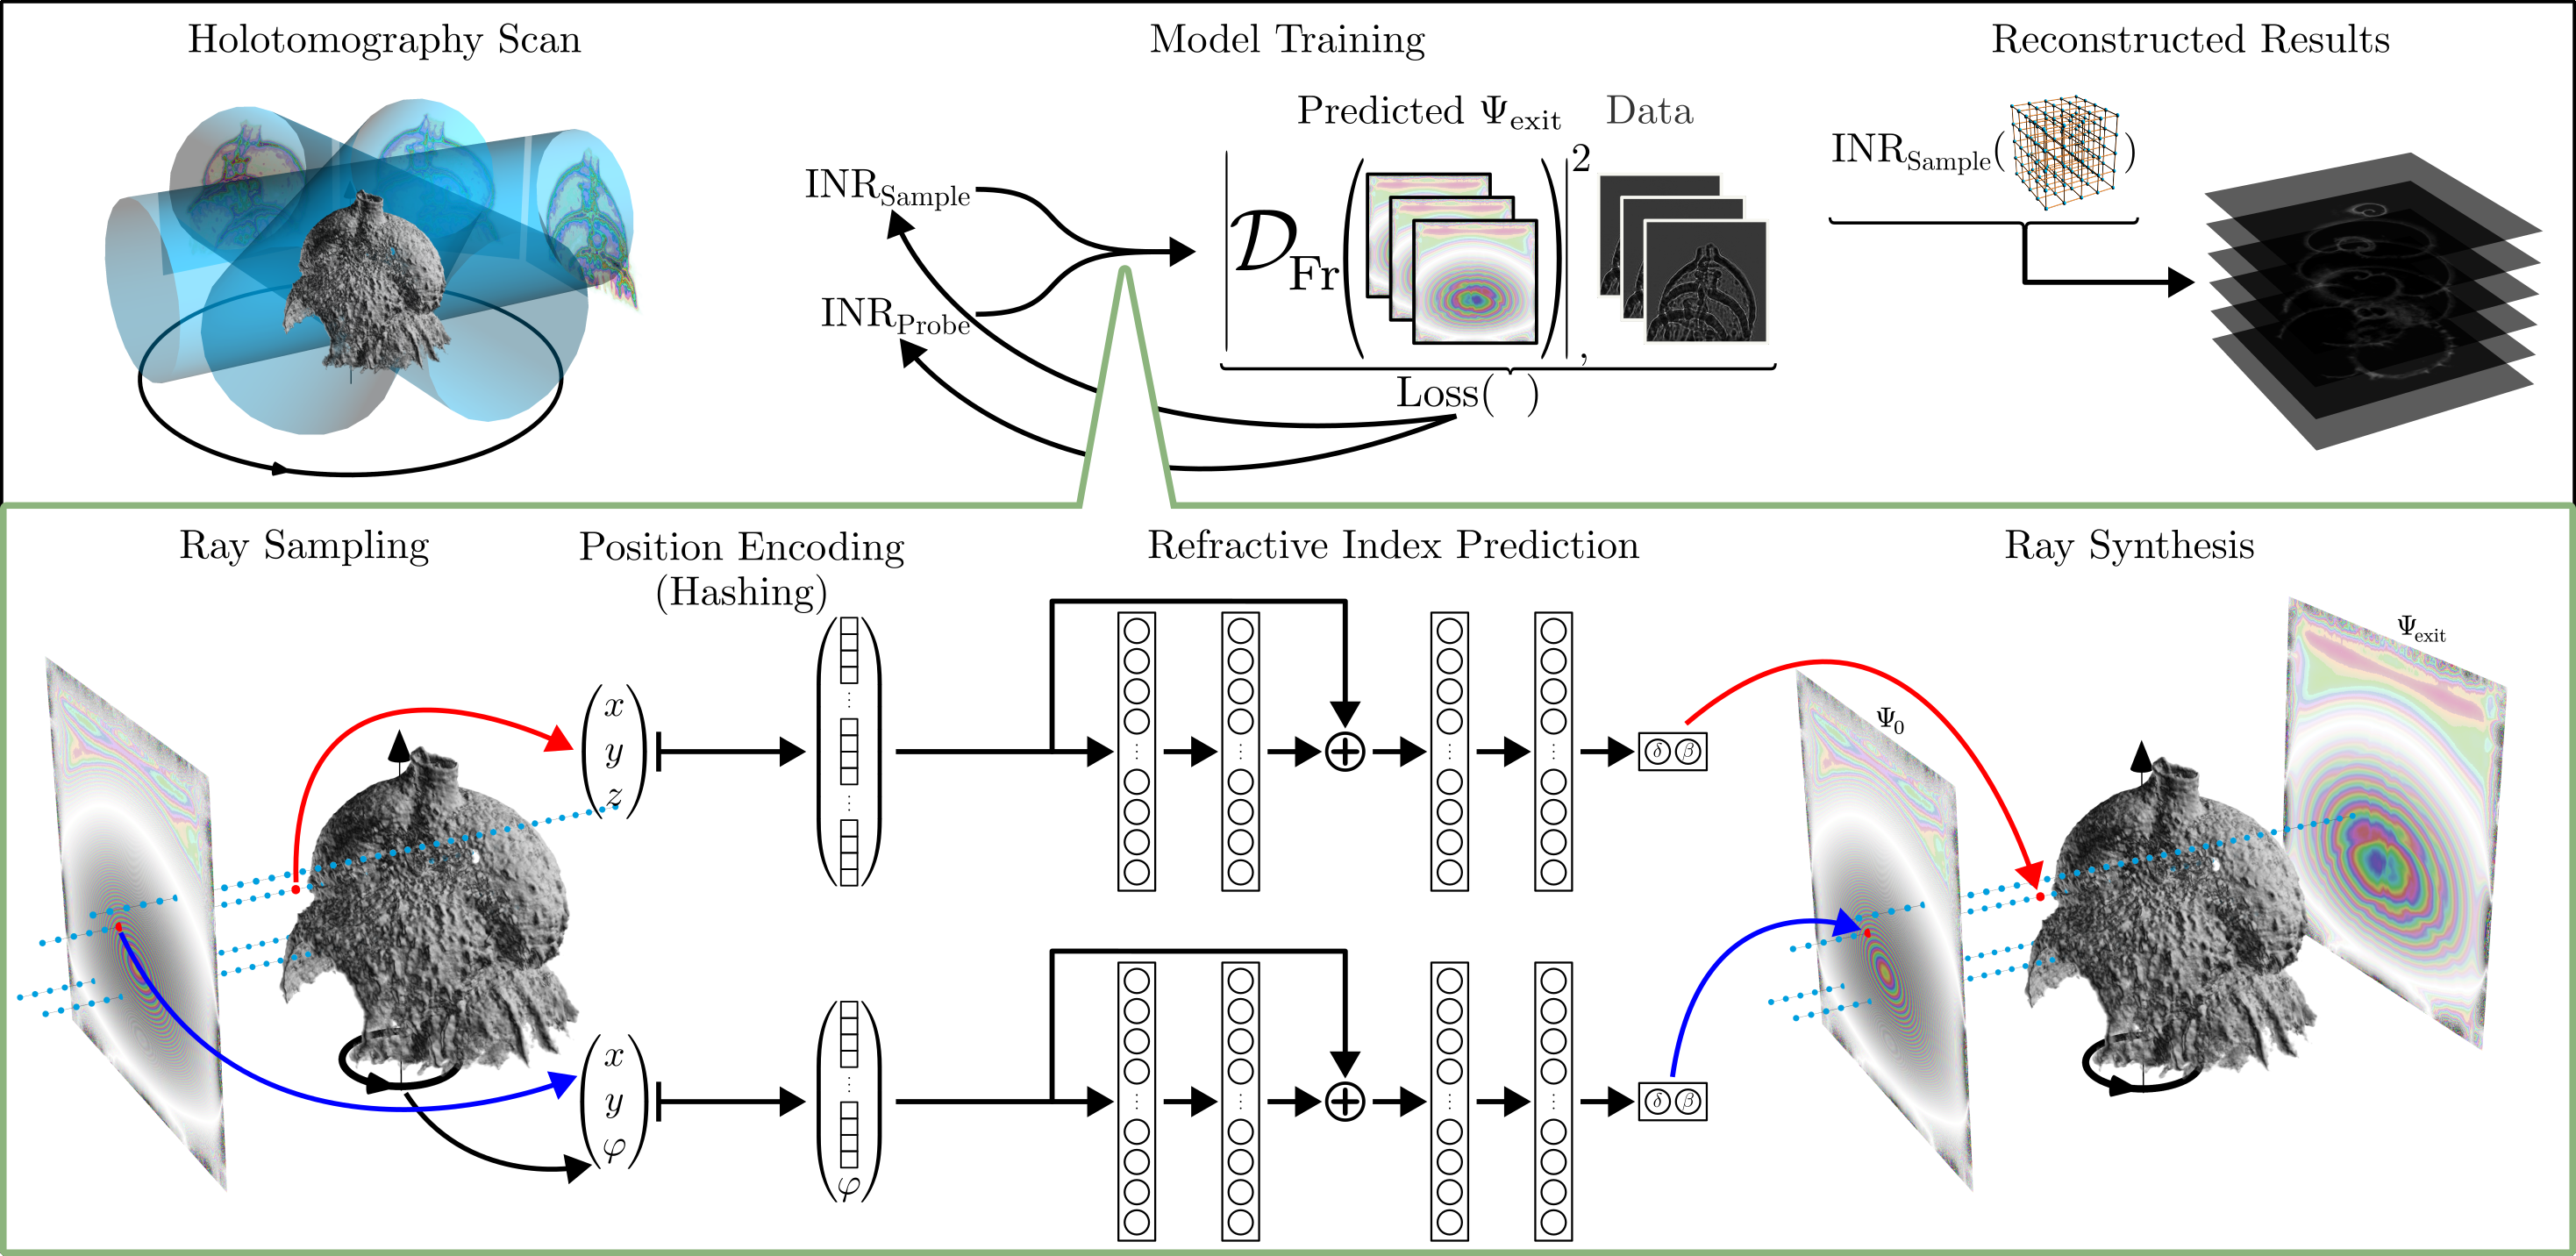
\includegraphics[width=1\linewidth]{images/overview.png}
	\caption{Left: Measurement process.
		Object is rotated while measuring, leading to angular dependent holograms.
		Center: Description of the ray sampling.
		For a given position the INR predicts phase and absorption, which is then integrated along the ray.
		Right: Training process.
		The resulting 2D image is then propagated to the detector and the model is trained by minimizing the loss.
	}
	\label{fig:overiew}
\end{figure*}

\subsection{Forward Model}
The interaction of X-rays with matter results in phase shifts and absorption, characterized by the complex refractive index of the material.
Therefore, the objective is to reconstruct the refractive index of the object  
\begin{align}
	O \left( x,y,z \right) = \delta \left( x,y,z \right) + \mathrm{i} \beta \left( x,y,z \right),
	\label{eq:refractive-index}
\end{align}
where $\delta \in \mathbb{R}_{\leq 0}$ denotes the phase shift and $\beta \in \mathbb{R}_{\geq 0}$ the absorption property at position $\left( x,y,z \right) \in \mathbb{R}^{3}$.  
The reconstruction is based on a set of measured intensities $\mathcal{I}_\varphi \left( x,y \right) \in \mathbb{R}_{\geq 0}$, where $\varphi \in \left[ 0, \pi \right)$ denotes the rotation angle of the object around the $y$-axis.  
The refractive index is linked to the measured intensity via the following forward model:

The interaction of the incoming wave field $\Psi_{0} \left( x,y \right)$ with the object is modeled as
\begin{align}
	\Psi_{\text{exit}, \varphi} \left( O \right) \left( x,y \right) =
	\exp \left( - \mathrm{i}k  \int_{\ell_{\varphi, x, y}} O \left( \x \right) \mathrm{d}\x \right) 
	\Psi_{0}\left( x,y \right),
\end{align}
where $\ell_{\varphi, x, y}$ denotes the line corresponding to a ray passing through the point $\left( x,y \right)$ at angle $\varphi$. This is commonly referred to as the thin-object approximation~\cite{paganinCoherentXrayOptics2006a}.  

Propagation of the wavefield through free space is described by the Fresnel approximation:  
\begin{align}
	\mathcal{D}_{\text{Fr}} \left( O \right) = 
	\mathcal{F}^{-1} \left[ 
		\exp \left( - \mathrm{i} \pi \frac{k_{x}^{2} + k_{y}^{2}}{\text{Fr}} \right) 
		\cdot \mathcal{F} \left( \Psi_{\text{exit}} \right)
	\right],
	\label{eq:fresnel}
\end{align}
where $\mathcal{F}$ and $\mathcal{F}^{-1}$ denote the Fourier transform and its inverse, and the Fresnel number $\text{Fr}$ characterizes the geometry of the experimental setup \cite{paganinCoherentXrayOptics2006a}.
While Fresnel propagation yields a complex-valued field, the detector can only record the corresponding intensities
\begin{align}
	\mathcal{I} = \left| \mathcal{D}_{\text{Fr}} \left( O \right) \right|^{2}.
\end{align}

\subsection{Implicit Neural Representation}
As depicted in Figure~\ref{fig:overiew}, the goal is to sample the object at positions $\left( x,y,z \right) \in \mathbb{R}^{3}$ and to integrate along the $z$-axis.  
The resulting projection is then Fresnel-propagated and compared to the measured intensities.  

In principle, a simple voxel grid could be employed, where all points are sampled explicitly.  
However, this approach results in a number of free variables scaling cubical with the size of the detector.  
In our case, this would correspond to approximately 16~billion model parameters, leading to severe computational and memory limitations.  

On the other hand, it is well known that volumetric samples typically consist of approximately uniform regions separated by sharp boundaries.  
Hence, neighboring voxels are strongly correlated, allowing a significant reduction in the number of parameters by exploiting this spatial redundancy.  
One way to achieve this is through a multilayer perceptron (MLP), which can theoretically approximate any continuous function.  
In practice, however, MLPs tend to favor low-frequency components, limiting their ability to represent fine details.  
This limitation has been mitigated by encoding schemes such as \emph{frequency encoding} and \emph{hash encoding}~\cite{mullerInstantNeuralGraphics2022,mildenhallNeRFRepresentingScenes2020a}.  
In this work, we adopt hash encoding, as it promotes smoother reconstructions compared to frequency encoding.  

Practically, hash encoding is implemented as follows:  
the volume is represented across $L$ resolution levels, i.e., $L$ voxel grids with increasing resolution.  
For a given level $l$ a coordinate $\mathbf{x} \in \mathbb{R}^{3}$ is scaled by the level's resolution, each surrounding grid point $\tilde{\mathbf{x}} \in \mathbb{Z}^{3}$ is mapped to a hash table entry as follows:
If the number of vertices at resolution $l$ is smaller than the hashtable size the mapping is one-to-one.
Otherwise it is mapped through a spatial hash function,
\begin{equation}
\begin{split}
h : \mathbb{Z}^{3} &\rightarrow \mathbb{Z}_{T} \\
\tilde{\mathbf{x}} &\mapsto \left( \bigoplus_{i=1}^{3} x_{i} \pi_{i} \right) \bmod T,
\end{split}
\end{equation}
where $\oplus$ denotes the bitwise XOR operation, $\pi_{1}=1$ and $\pi_{i}$ are large, distinct prime numbers, and $T$ is the hash table size.  
The feature value at position $\mathbf{x}$ is obtained via trilinear interpolation of the hash tables entries.  
This process is repeated for all levels, and the resulting multi-resolution features are concatenated and fed into the MLP, which then predicts absorption and phase for a given input.
Per level $l$ a hash table with size $T$ and $F$ feature channels is learned.  
For further details, we refer to Müller~\textit{et~al.}~\cite{mullerInstantNeuralGraphics2022}.  

\subsection{Optimization}
During the training we minimize the loss function 
\begin{equation}
	\begin{split}
\mathcal{L}\!\left( O_{\mathrm{pred}}, \mathcal{I}_\varphi \right)
 = &\, 
 \left\|
 \left|
 \mathcal{D}_{\mathrm{Fr}}\!\left(
 \Psi_{\mathrm{exit}, \varphi}\!\left(
 O_{\mathrm{pred}}
 \right)
 \right)
 \right|
 -
 \sqrt{\mathcal{I}_\varphi}
 \right\|_{L_{2}}^{2} \\[0.5em]
   & + \alpha\, \mathrm{TV}\!\left(
 \Psi_{\mathrm{exit}, \varphi}\!\left(
 O_{\mathrm{pred}}
 \right)
 \right),
 \label{eq:loss}
\end{split}
\end{equation}
where $\alpha \in \mathbb{R}_{+}^{2}$, and the total variation norm is computed independently for the real and imaginary parts of $\Psi_{\mathrm{exit}, \varphi}\!\left( \tilde{O}_{\mathrm{pred}} \right)$.  
 
Training is performed using the AdamW optimizer with a learning-rate of \num{e-2} and a learning-rate scheduler that halves the rate if the loss does not improve for $300$ angles \cite{loshchilovDecoupledWeightDecay2019}.
The training is stopped after $4000$ steps or if the learning-rate is below \num{e-5}.


\subsection{Implementation Details}
As hyperparameters for the hash encoding, we choose $T = 2^{21}$, $F = 4$, and $L = 16$, which have empirically shown good results.  
The output of the hash encoding is a vector of length $64$.  
The MLP consists of four layers with 64 neurons each and includes a skip connection from the hash encoding output to the output of the second layer.  
The final layer maps the 64-dimensional feature space to two output channels, representing phase and absorption.  
Leaky ReLU activations are used after each hidden layer.  
The final layer squares its output to enforce non-negativity of the phase and absorption component.  

This results in a total memory footprint of \qty{441}{\mega\byte} compared to \qty{64}{\gibi\byte} for a cubic $2048^3$ grid with complex values, corresponding to a compression of approximately $95\%$.  

To fully sample the Fresnel operator, it has been shown that $N > \frac{1}{\mathrm{Fr}}$ samples are required~\cite{paganinCoherentXrayOptics2006a}.  
Therefore, the MLP is sampled at each rotation angle along rays on a grid of $N \times N$, with each ray discretized into $N$ points.  
The rays are then integrated and discretized to perform Fresnel propagation.  
\section{Experimental Details}
Measurements were conducted at beamline P05 at PETRA~III, located at DESY (Hamburg, Germany) operated by Helmholtz-Center Hereon.
A Fresnel-zone-plate based setup was used as described by Flenner~\cite{flennerHardXrayNanoholotomography2020b}.
For demonstration purpose we chose a foraminifera sample, measured at 1584 angles with a Fresnel-number of \num{9.979e-4} at \qty{17}{\keV}~\cite{niEarlyDiagenesisForaminiferal2020}.
We compare our proposed approach to a two step approach consisting of a state of the art phase-retrieval algorithm and filtered back projection and evaluate how many angles are necessary for reconstruction~\cite{doraArtifactsuppressingReconstructionStrongly2024}.
The input holograms are flat-field corrected as described in Dora~\textit{et~al.}~\cite{doraArtifactsuppressingReconstructionStrongly2024}.



\vfill\pagebreak

\label{sec:refs}
\bibliographystyle{IEEEbib}
\bibliography{refs}

\end{document}
